%!TEX root = ../Project.tex

\section{Implementation}

\subsection{Overview}

\begin{figure}[htbp]
	\centering
		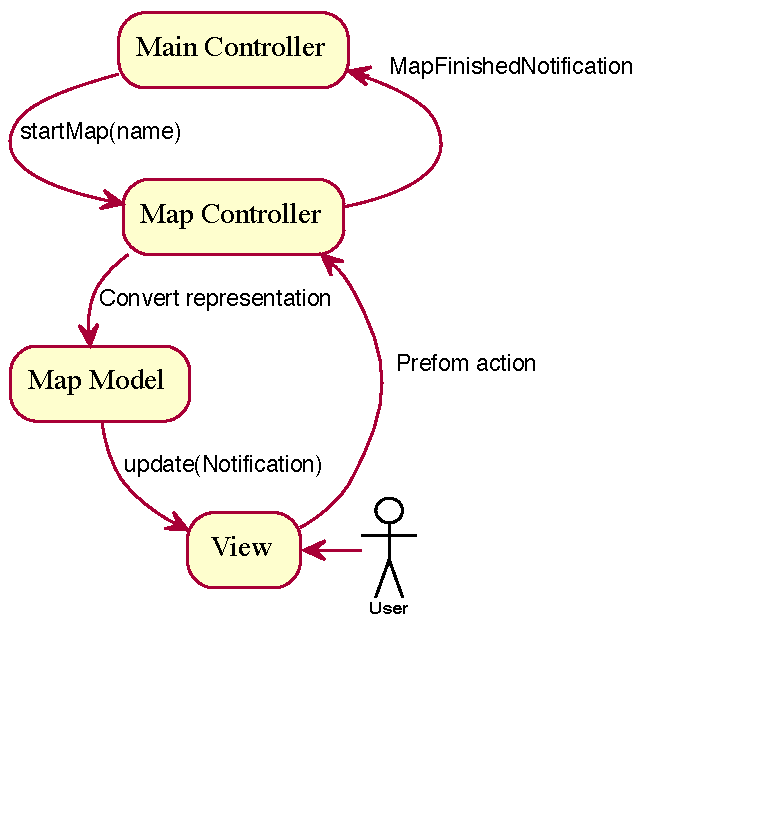
\includegraphics{figures/engine_exported.pdf}
	\caption{caption}
	\label{fig:Overview of the engine}
\end{figure}

The system is structures using MVC for the overall archavice as well as  using the Observer Patten as shown  above.


The \texttt{MainController} handles the overall logic, inducing the game progression. 
Although the objectives only required a isometric  map view, the archavice was designed to be more general. Hence a \emph{separate} controller for each part of the game is used. When the part is  (e.g. when a map has been completed) the controller notifies the \texttt{MainController}, which decides what to do next.   

%TODO where to put?
The archavive could be easily extended to overworld maps, cut-scenes for example.


The obsverable components (i.e the view, or the map controller) commimite using \texttt{notification} object. 


\subsection{Engine Development and Testing}
\label{sub:engine_development_and_testing}

\subsubsection{Data Format}


\subsubsection{Maps}
\label{ssub:maps}

\subsubsection{Units}
\label{ssub:units}

\subsubsection{Events}
\label{ssub:events}

\subsubsection{Algorithms}
\label{ssub:Algorithms}

\subsubsection{Inter-compatibility}
\label{ssub:intercompatibility}
As discussed previously the maps use xml as their data format, one the advantages of this was that it required very little changes to the data format to have incompatibility with Oleksandr Stasyk's  Terrain Generator's output format.  The Terrain generator allows uses various algorithms to produce senabient looking map. Users can use these as a starting  point, to make it for them to design their maps.


\subsection{Gui Development and Testing}

\subsubsection{Map Rendering}
\label{ssub:map_rendering}

\subsection{User Interface}


\subsubsection{Custom Classes} % allows user to use their own code
\label{ssub:custom_classes}


\subsection{Editor Development and Testing}

\subsubsection{Overview}
\label{ssub:overview}

\subsubsection{Map Editor}
\label{ssub:map_editor}

\subsubsection{Unit Editor}
\label{ssub:unit_editors}

\subsubsection{Event Editing}

\subsubsection{Exporting}
\label{ssub:exporting}

The editor can export the game as a complete package, either as a Mac OS X application or as jar. These application don't require any external resources, apart from a recent version of java\footnote{specifically Java 1.6+}.

A prominent feature of the editor is that the jar will work on any Java enabled platform, since the jar contains all required libraries for each platform. The OS X application can even be exported on other platforms.

While most of the testing was done on OS X \footnote{Mac OS X 10.6 Snow leopard}, it also works well on Linux \footnote{Science  Linux x.y}. It even has limited compatibly with Windows\footnote{Tested on Windows 7 32 bit} (apart from some minor graphics issues).
